\documentclass{article}

\usepackage{tikz}
\usetikzlibrary{calc,backgrounds}
%\usepackage[active,tightpage]{preview}

\begin{document}

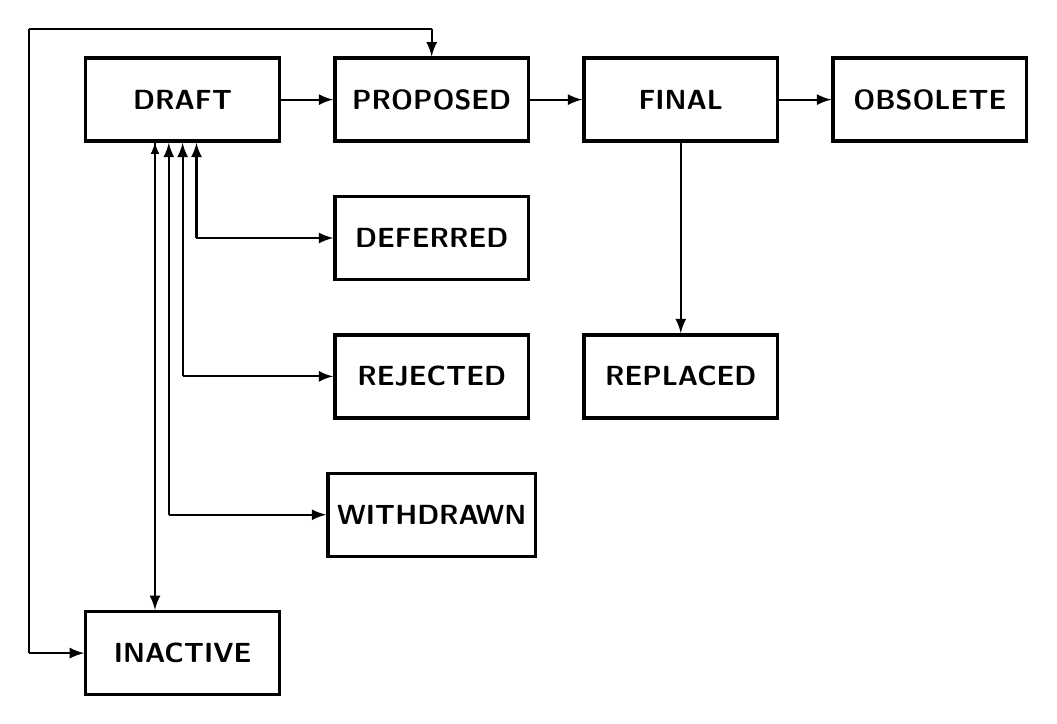
\begin{tikzpicture}[>=latex]

  \tikzstyle{state} = [draw, very thick, fill=white, rectangle, minimum height=3em, minimum width=7em, node distance=5em, font={\sffamily\bfseries}]
  \tikzstyle{stateEdgePortion} = [black,thick];
  \tikzstyle{stateEdge} = [stateEdgePortion,->];
  \tikzstyle{edgeLabel} = [pos=0.5, text centered, font={\sffamily\small}];

  \node[state, name=draft] {DRAFT};
  \node[state, name=inactive, below of=draft, yshift=-15em] {INACTIVE};
  \node[state, name=proposed, right of=draft, xshift=4em] {PROPOSED};
  \node[state, name=deferred, below of=proposed] {DEFERRED};
  \node[state, name=rejected, below of=deferred] {REJECTED};
  \node[state, name=withdrawn, below of=rejected] {WITHDRAWN};
  \node[state, name=final, right of=proposed, xshift=4em] {FINAL};
  \node[state, name=replaced, right of=rejected, xshift=4em] {REPLACED};
  \node[state, name=obsolete, right of=final, xshift=4em] {OBSOLETE};

  % Drafts can become inactive, and inactive states can go back to drafts
  \draw[<->] ($(draft.south) + (-1em,0)$)
    edge[stateEdge] ($(inactive.north) + (-1em,0)$);

  % Drafts can become proposed
  \draw ($(draft.east)$)
    edge[stateEdge] ($(proposed.west)$);

  % Drafts can become withdrawn, and withdrawn can go back to being drafts
  \coordinate (draftWithdrawnA) at ($(withdrawn.west -| draft.south) + (-0.5em,0)$);
  \draw (draftWithdrawnA) edge[stateEdge] ($(draft.south) + (-0.5em,0)$);
  \draw (draftWithdrawnA) edge[stateEdge] ($(withdrawn.west)$);
  
  % Drafts can become rejected, and rejected can go back to being drafts
  \coordinate (draftRejectedA) at ($(rejected.west -| draft.south)$);
  \draw (draftRejectedA) edge[stateEdge] ($(draft.south)$);
  \draw (draftRejectedA) edge[stateEdge] ($(rejected.west)$);

  % Drafts can become deferred, and deferred can go back to being drafts
  \coordinate (draftDeferredA) at ($(deferred.west -| draft.south) + (0.5em,0)$);
  \draw (draftDeferredA) edge[stateEdge] ($(draft.south) + (0.5em,0)$);
  \draw (draftDeferredA) edge[stateEdge] ($(deferred.west)$);

  % Proposed can become final/active
  \draw ($(proposed.east)$)
    edge[stateEdge] ($(final.west)$);

  % Final/active can become obsolete
  \draw ($(final.east)$)
    edge[stateEdge] ($(obsolete.west)$);

  % Final/active can also become replaced
  \draw ($(final.south)$)
    edge[stateEdge] ($(replaced.north)$);

  % Proposed can become inactive, and inactive can return to proposed
  \coordinate (proposedInactiveA) at ($(proposed.north) + (0,1em)$);
  \coordinate (proposedInactiveB) at ($(proposed.north -| draft.west) + (-2em,1em)$);
  \coordinate (proposedInactiveC) at ($(inactive.west) + (-2em,0)$);
  \draw (proposedInactiveA) edge[stateEdge] (proposed.north);
  \draw (proposedInactiveA) edge[stateEdgePortion] (proposedInactiveB);
  \draw (proposedInactiveB) edge[stateEdgePortion] (proposedInactiveC);
  \draw (proposedInactiveC) edge[stateEdge] ($(inactive.west)$);

\end{tikzpicture}

\end{document}
